\documentclass[conference]{IEEEtran}
\IEEEoverridecommandlockouts

\usepackage{cite}
\usepackage{amsmath,amssymb,amsfonts}
\usepackage{graphicx}
\graphicspath{{figures/}}
\usepackage{booktabs}
\usepackage{siunitx}
\usepackage{textcomp}
\usepackage{xcolor}

\sisetup{group-separator={,}, group-minimum-digits=4}

\begin{document}

\title{Exploratory Data Analysis of a Car Insurance Claim Dataset}

% TODO: replace with your team's names and details
\author{
\IEEEauthorblockN{Brian Chin}
\IEEEauthorblockA{\textit{Department of Computer Science and Engineering} \\
\textit{University at Buffalo}\\
Buffalo, NY, USA \\
bschin@buffalo.edu}
}

\maketitle

\begin{abstract}
\end{abstract}

\begin{IEEEkeywords}
\end{IEEEkeywords}

\section{Introduction}

\section{Mean, Median, and Mode Analysis}

For CREDIT\_SCORE, the mean (0.516) and median (0.526) are very close, and the skewness is only $-0.23$. This 
means the distribution is almost symmetric with a small left tail, so both the mean and median are good summaries.

The mode of CREDIT\_SCORE is not very useful. The column has \num{9026} unique values across \num{10000} rows, 
so almost every driver has a different score. The mode is 0.5795, which shows up 324 times, but this value comes from the 
regression imputation we used to fill missing scores rather than from a real cluster of drivers. Because of this, we did 
not report a mode for credit score in Table~\ref{tab:numeric}. 
 
ANNUAL\_MILEAGE is also close to symmetric (skew = 0.04), and its mean (\num{11698}), median (\num{12000}), 
and mode (\num{11000}) are all close together. Here the mode does make sense, because mileage is mostly recorded in 
steps of \num{1000} miles (there are only 62 unique values), and \num{11000} is the most common value, appearing \num{1253} 
times. Any of the three statistics would be a reasonable summary of a typical driver's mileage.

\begin{table}[t]
\caption{Descriptive Statistics for Continuous and Count Features}
\label{tab:numeric}
\centering
\begin{tabular}{@{}lrrrr@{}}
\toprule
\textbf{Feature} & \textbf{Mean} & \textbf{Median} & \textbf{Mode} & \textbf{Skew} \\
\midrule
\multicolumn{5}{@{}l}{\textit{Continuous}} \\
CREDIT\_SCORE        & 0.516       & 0.526       & ---         & $-0.23$ \\
ANNUAL\_MILEAGE      & \num{11698} & \num{12000} & \num{11000} & 0.04 \\
INSURANCE\_RISK      & 0.099       & 0.071       & 0           & 1.71 \\
\midrule
\multicolumn{5}{@{}l}{\textit{Count}} \\
SPEEDING\_VIOLATIONS & 1.48        & 0           & 0           & \multicolumn{1}{c}{\textsuperscript{a}} \\
DUIS                 & 0.24        & 0           & 0           & \multicolumn{1}{c}{\textsuperscript{a}} \\
PAST\_ACCIDENTS      & 1.06        & 0           & 0           & \multicolumn{1}{c}{\textsuperscript{a}} \\
\bottomrule
\multicolumn{5}{@{}p{0.95\columnwidth}@{}}{\footnotesize \textsuperscript{a}Skewness of the count features ranges from approximately 2.15 to 2.76.}
\end{tabular}
\end{table}

The count variables exhibit even stronger right skew. SPEEDING\_VIOLATIONS, DUIS, and PAST\_ACCIDENTS each have a median and mode of 0, while their means are 1.48, 0.24, and 1.06, respectively. Their skewness values range from approximately 2.15 to 2.76. This pattern indicates that most drivers have no recorded violations, DUIs, or past accidents, whereas a smaller group has multiple incidents. The mean alone therefore overstates the incident count of a typical driver; the median and mode provide essential complementary information.

For binary variables, the mean equals the proportion of observations in class~1 (Table~\ref{tab:binary}). 
Approximately 69.7\% of observations have VEHICLE\_OWNERSHIP $=1$, and MARRIED is nearly balanced at 
49.8\%. CHILDREN and the engineered FAMILY feature have class-1 proportions of 68.8\% and 77.7\%, respectively.

For the target, OUTCOME has a mean of 0.313, so 31.3\% of drivers filed a claim and 68.7\% did not. This 
imbalance is important for modeling. A model that always predicts ``no claim'' would already get about 68.7\% accuracy, 
so we plan to also look at precision, recall, and F1-score instead of only accuracy.
 
\begin{table}[t]
\caption{Class-1 Proportions for Binary Features}
\label{tab:binary}
\centering
\begin{tabular}{@{}lr@{}}
\toprule
\textbf{Feature} & \textbf{Proportion in Class 1} \\
\midrule
VEHICLE\_OWNERSHIP     & 0.697 \\
MARRIED                & 0.498 \\
CHILDREN               & 0.688 \\
FAMILY (engineered)    & 0.777 \\
\midrule
OUTCOME (target)   & 0.313 \\
\bottomrule
\end{tabular}
\end{table}

For categorical features, Table~\ref{tab:categorical} shows the most common category, its percentage, and the second 
most common category. Two features are almost constant: VEHICLE\_TYPE is 95.2\% sedan and RACE is 
90.1\% majority. Features like these probably will not help a model much because almost every row has the same value. 
VEHICLE\_YEAR (69.7\% before 2015) and POSTAL\_CODE (69.4\% in one code) are also dominated by one 
value, but less extremely.
 
Other features are more balanced. GENDER is almost evenly split, and for AGE, 
DRIVING\_EXPERIENCE, EDUCATION, and INCOME, the top category is not much bigger than the 
second one. CAR\_AGE is 50.9\% ``Old'', partly because of how we defined it: two of the four rules we used 
map to ``Old''. AGE\_GROUP and EXPERIENCE\_LEVEL have the same mode percentages as AGE and 
DRIVING\_EXPERIENCE (30.6\% and 35.3\%) since they are just relabeled versions.
 
\begin{table}[t]
\caption{Mode and Second Most Common Category for Categorical Features}
\label{tab:categorical}
\centering
\setlength{\tabcolsep}{3pt}
\begin{tabular}{@{}llrlr@{}}
\toprule
\textbf{Feature} & \textbf{Mode} & \textbf{\%} & \textbf{2nd} & \textbf{\%} \\
\midrule
VEHICLE\_TYPE  & sedan       & 95.2 & sports car   & 4.8 \\
RACE           & majority    & 90.1 & minority     & 9.9 \\
VEHICLE\_YEAR  & before 2015 & 69.7 & after 2015   & 30.3 \\
POSTAL\_CODE   & 10238       & 69.4 & 32765        & 24.6 \\
CAR\_AGE       & Old         & 50.9 & Very Old     & 29.2 \\
GENDER         & female      & 50.1 & male         & 49.9 \\
INCOME         & upper class & 43.4 & middle class & 21.4 \\
EDUCATION      & high school & 41.6 & university   & 39.3 \\
DRIVING\_EXP.  & 0--9y       & 35.3 & 10--19y      & 33.0 \\
AGE            & 26--39      & 30.6 & 40--64       & 29.3 \\
\bottomrule
\end{tabular}
\end{table}

\section{Chi-Square Test Analysis}
We used the chi-square test of independence to check whether each categorical feature is related to OUTCOME. 
This test works here because both the features and the target are categories, so we cannot use a normal correlation. 
For each of the 12 categorical features, the null hypothesis $H_0$ is that the feature and OUTCOME are 
independent. We used a significance level of $\alpha = 0.05$.
 
The chi-square test needs every expected cell count to be at least 5. The smallest expected count in all of our tests 
was 37.6, so this assumption is satisfied and we did not have to combine any categories. The results are in 
Table~\ref{tab:chi2}, sorted by $\chi^2$.

Ten of the twelve features have $p < 0.05$, so we reject $H_0$ for them. Driving experience ($\chi^2 = 2809.9$) and age 
($\chi^2 = 2308.8$) have by far the strongest relationship with filing a claim, followed by income ($\chi^2 = 1798.0$). 
We sorted by $\chi^2$ instead of $p$-value because with \num{10000} rows, the top five $p$-values all came out as 0 and 
could not be compared. One thing to keep in mind is that $\chi^2$ also gets bigger with more degrees of freedom, so this 
ranking is only a rough comparison.

\begin{table}[t]
\caption{Chi-Square Test Results Against OUTCOME}
\label{tab:chi2}
\centering
\setlength{\tabcolsep}{4pt}
\begin{tabular}{@{}lrrrr@{}}
\toprule
\textbf{Feature} & $\boldsymbol{\chi^2}$ & \textbf{dof} & $\boldsymbol{p}$\textbf{-value} & \textbf{Min.\ exp.} \\
\midrule
DRIVING\_EXP.      & 2809.9 & 3 & 0.0\textsuperscript{b}  & 329.6 \\
EXPERIENCE\_LEVEL  & 2806.5 & 2 & 0.0\textsuperscript{b}  & 993.5 \\
AGE                & 2308.8 & 3 & 0.0\textsuperscript{b}  & 623.5 \\
AGE\_GROUP         & 2308.8 & 3 & 0.0\textsuperscript{b}  & 623.5 \\
INCOME             & 1798.0 & 3 & 0.0\textsuperscript{b}  & 536.4 \\
CAR\_AGE           & 1046.7 & 2 & $5.1\times10^{-228}$ & 624.4 \\
VEHICLE\_YEAR      & 864.0  & 1 & $6.5\times10^{-190}$ & 950.2 \\
POSTAL\_CODE       & 388.1  & 3 & $8.3\times10^{-84}$  & 37.6 \\
EDUCATION          & 365.4  & 2 & $4.6\times10^{-80}$  & 600.0 \\
GENDER             & 114.5  & 1 & $1.0\times10^{-26}$  & 1563.4 \\
\midrule
RACE               & 0.6    & 1 & 0.428 & 309.5 \\
VEHICLE\_TYPE      & 0.3    & 1 & 0.609 & 149.4 \\
\bottomrule
\multicolumn{5}{@{}p{0.95\columnwidth}@{}}{\footnotesize \textsuperscript{b}Python returned 0 because the value is too small to store as a float.}
\end{tabular}
\end{table}
 
We also noticed some things about our engineered features. AGE\_GROUP has exactly the same result as AGE, 
which is expected since it is just a renamed version. EXPERIENCE\_LEVEL combines the two most experienced groups 
into one, but its $\chi^2$ (2806.5) is almost the same as DRIVING\_EXPERIENCE (2809.9). This means combining 
those groups did not lose much information. Since each pair is really the same variable, we should consider to keep one 
from each pair when building our model.
 
RACE ($\chi^2 = 0.6$, $p = 0.428$) and VEHICLE\_TYPE ($\chi^2 = 0.3$, $p = 0.609$) are not significant, 
so we fail to reject $H_0$ for them. Since we have \num{10000} rows, the test has enough data to find even small effects, 
so this result suggests that these two features really are not related to claims. For example, the claim rates for the 
two RACE groups are 31.2\% and 32.5\%, which are very close. These two features were also almost constant in 
Table~\ref{tab:categorical}, so they are good candidates to drop.
 
\begin{figure}[t]
\centering
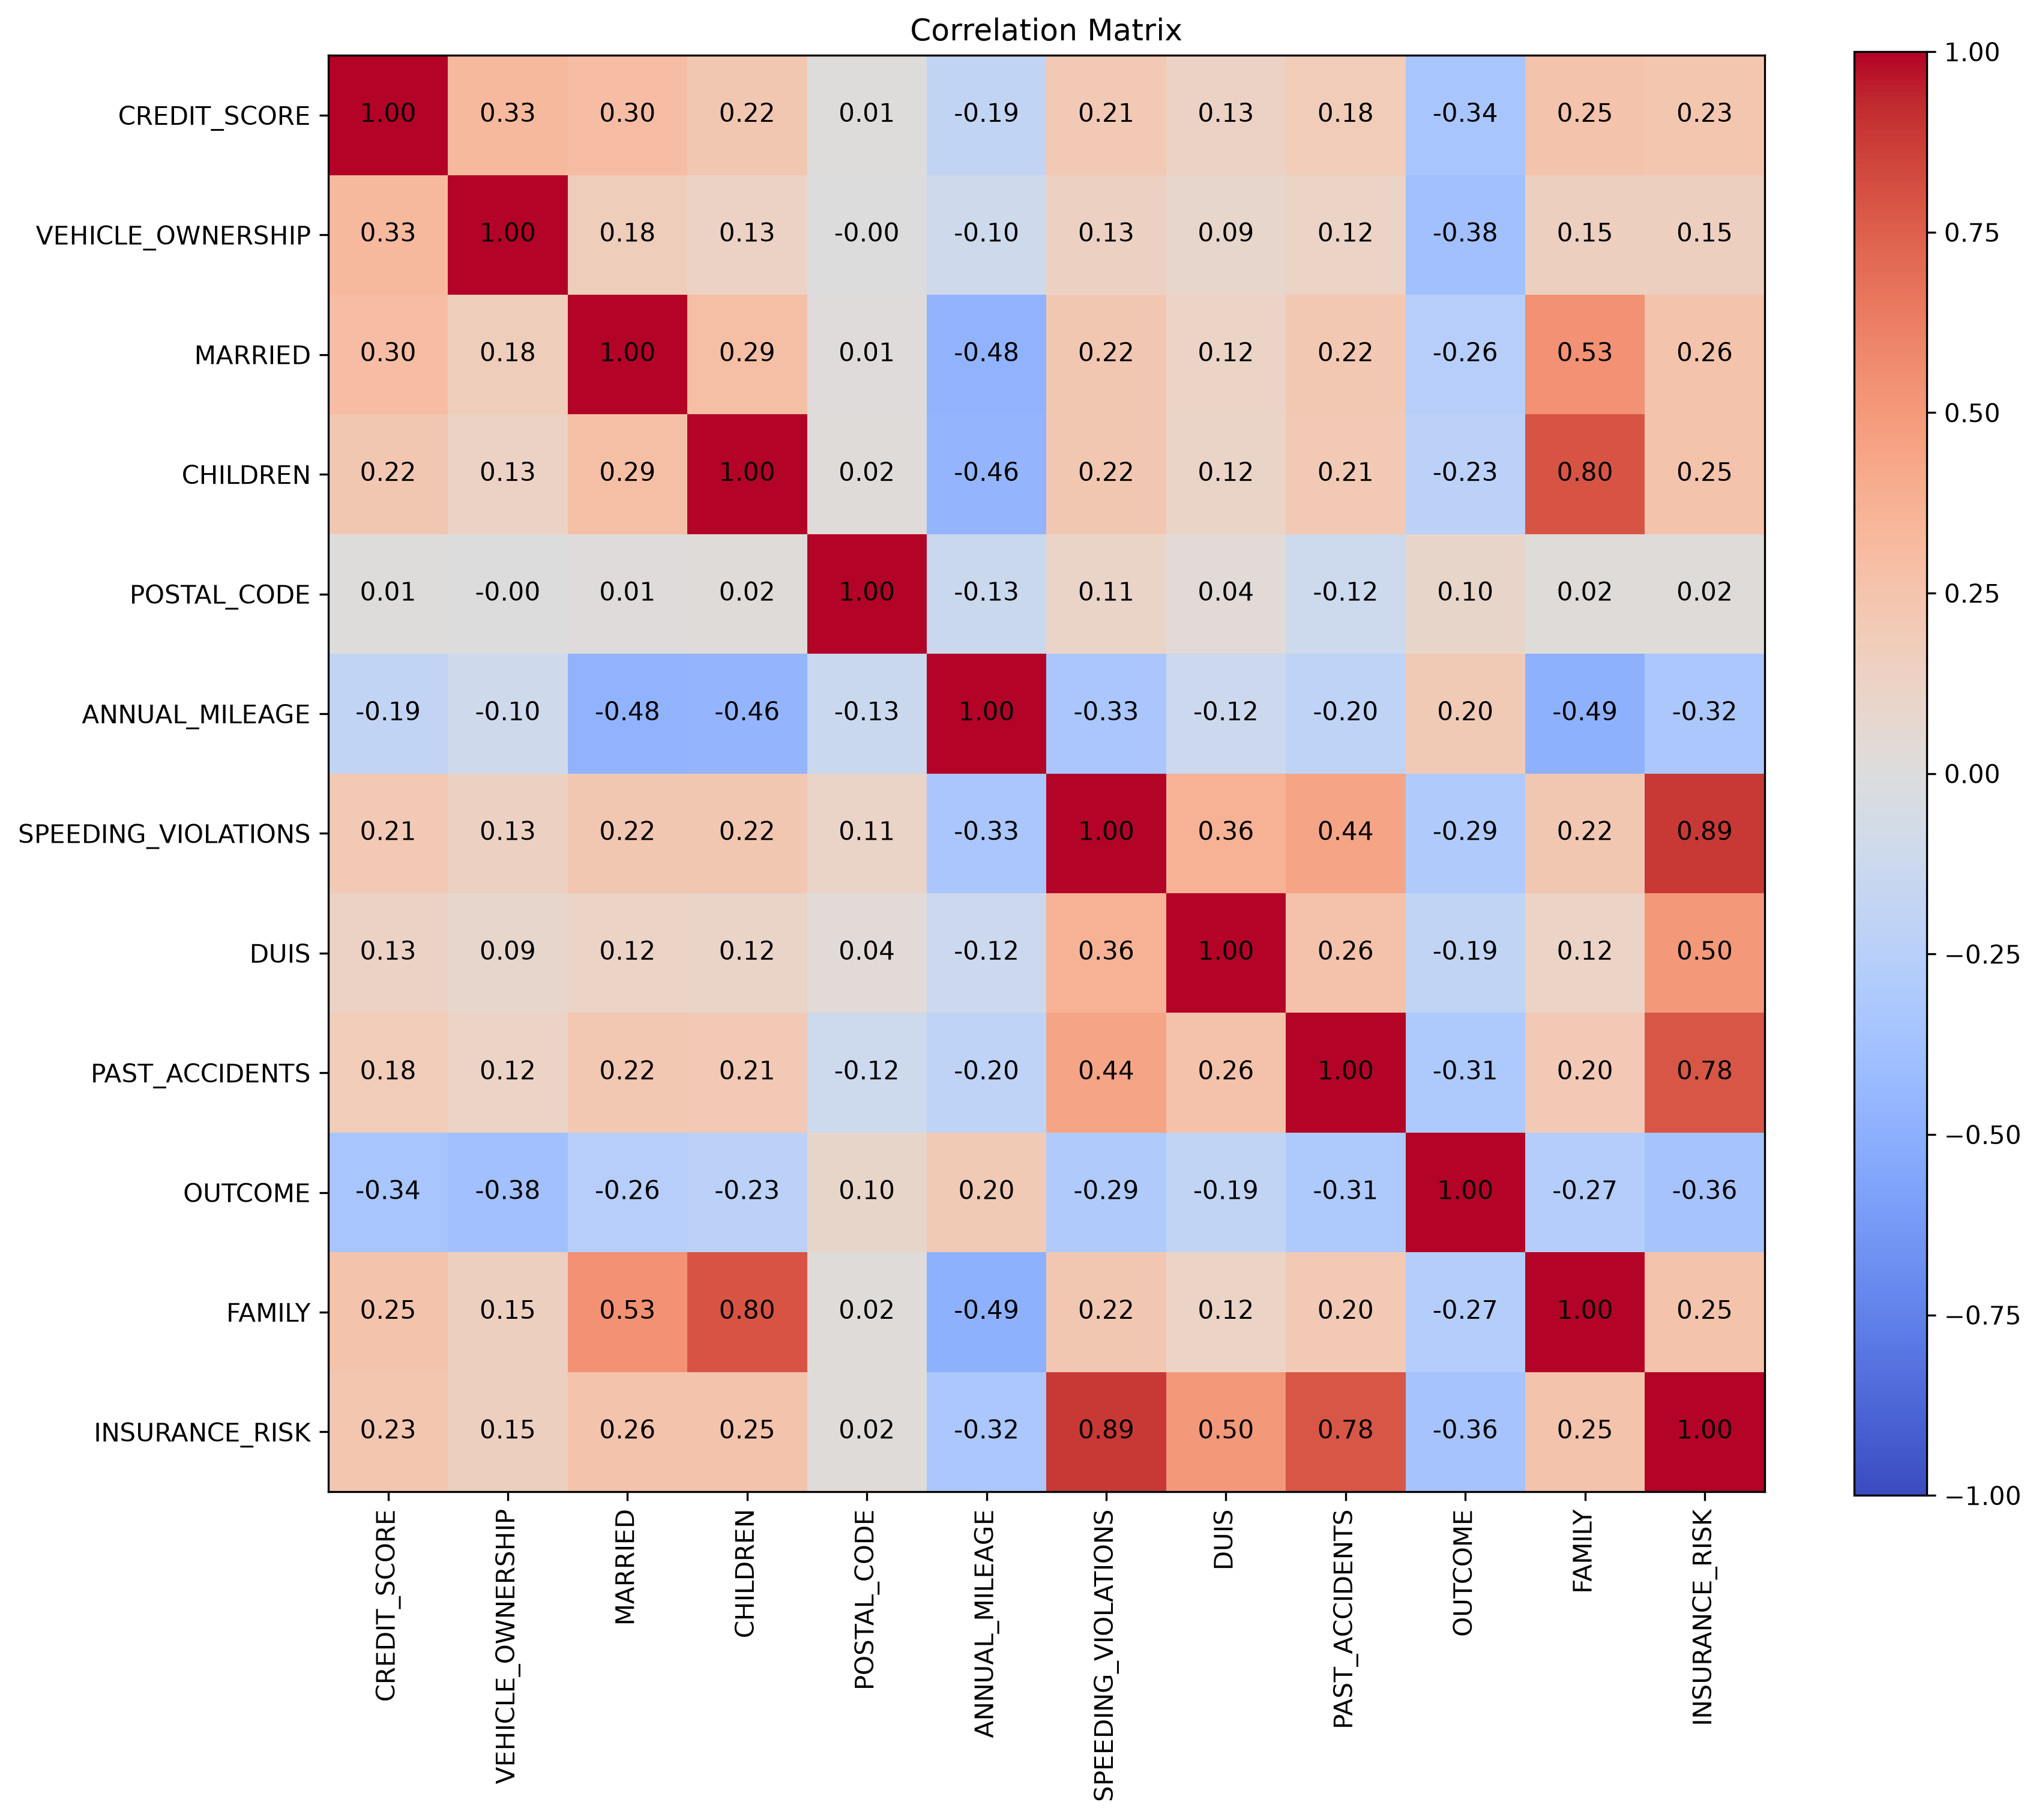
\includegraphics[width=\columnwidth]{corr.png}
\caption{Correlation matrix of the numeric features after preprocessing.}
\label{fig:corr}
\end{figure}

\section{Correlation Matrix Analysis}
The correlation matrix shows the Pearson correlation $r$ between each pair of numeric features. 
The value of $r$ goes from $-1$ to $+1$ and measures how strong the \emph{linear} relationship is. 
Fig.~\ref{fig:corr} shows the matrix for the preprocessed data. Since OUTCOME is binary, its 
correlation with a feature basically tells us how different that feature's average is between drivers 
who claimed and drivers who did not. POSTAL\_CODE shows up in the matrix because it is stored 
as a number, but we ignored its correlations since the number itself has no meaning.

\begin{table}[t]
\caption{Correlation of Numeric Features with OUTCOME}
\label{tab:corr_target}
\centering
\begin{tabular}{@{}lr@{}}
\toprule
\textbf{Feature} & $\boldsymbol{r}$ \\
\midrule
VEHICLE\_OWNERSHIP   & $-0.38$ \\
INSURANCE\_RISK      & $-0.36$ \\
CREDIT\_SCORE        & $-0.34$ \\
PAST\_ACCIDENTS      & $-0.31$ \\
SPEEDING\_VIOLATIONS & $-0.29$ \\
FAMILY               & $-0.27$ \\
MARRIED              & $-0.26$ \\
CHILDREN             & $-0.23$ \\
DUIS                 & $-0.19$ \\
ANNUAL\_MILEAGE      & $+0.20$ \\
\bottomrule
\end{tabular}
\end{table}

Table~\ref{tab:corr_target} lists each numeric feature's correlation with OUTCOME. All of them 
are weak to moderate ($|r| \le 0.38$), so no single numeric feature can predict claims well by itself. 
VEHICLE\_OWNERSHIP has the strongest correlation ($r = -0.38$), meaning drivers who own their car 
are less likely to file a claim. Next are INSURANCE\_RISK ($r = -0.36$) and CREDIT\_SCORE 
($r = -0.34$). ANNUAL\_MILEAGE is the only positive one ($r = 0.20$), so drivers who drive more tend 
to file claims a bit more often.

One result surprised us. SPEEDING\_VIOLATIONS ($r = -0.29$), PAST\_ACCIDENTS ($r = -0.31$), 
DUIS ($r = -0.19$), and INSURANCE\_RISK are all \emph{negatively} correlated with OUTCOME. 
In other words, drivers with more incidents on record are \emph{less} likely to have a claim in this dataset, which 
is the opposite of what we expected. 

\begin{table}[t]
\caption{Strongest Correlations Between Predictor Pairs}
\label{tab:corr_pairs}
\centering
\setlength{\tabcolsep}{4pt}
\begin{tabular}{@{}llr@{}}
\toprule
\textbf{Feature 1} & \textbf{Feature 2} & $\boldsymbol{r}$ \\
\midrule
SPEEDING\_VIOL.  & INSURANCE\_RISK  & $0.89$ \\
CHILDREN         & FAMILY           & $0.80$ \\
PAST\_ACCIDENTS  & INSURANCE\_RISK  & $0.78$ \\
MARRIED          & FAMILY           & $0.53$ \\
DUIS             & INSURANCE\_RISK  & $0.50$ \\
ANNUAL\_MILEAGE  & FAMILY           & $-0.49$ \\
ANNUAL\_MILEAGE  & MARRIED          & $-0.48$ \\
ANNUAL\_MILEAGE  & CHILDREN         & $-0.46$ \\
SPEEDING\_VIOL.  & PAST\_ACCIDENTS  & $0.44$ \\
\bottomrule
\end{tabular}
\end{table}

Table~\ref{tab:corr_pairs} shows the strongest correlations between predictor features. The highest ones are all 
between our engineered features and the columns they came from, such as INSURANCE\_RISK with 
SPEEDING\_VIOLATIONS ($r = 0.89$) and FAMILY with CHILDREN ($r = 0.80$). This is expected, 
but it means that if we keep both an engineered feature and its original columns, we will have multicollinearity. This 
is mostly a problem for linear and logistic regression, because the coefficients become unstable and hard to interpret. 
 
For the original features, ANNUAL\_MILEAGE is moderately negatively correlated with MARRIED ($r = -0.48$) 
and CHILDREN ($r = -0.46$), so married drivers and drivers with kids tend to drive less. 
SPEEDING\_VIOLATIONS and PAST\_ACCIDENTS are also moderately related ($r = 0.44$). 
CREDIT\_SCORE has a weak to moderate correlation with VEHICLE\_OWNERSHIP ($r = 0.33$) and MARRIED 
($r = 0.30$).

\begin{table}[t]
\caption{Strongest One-Hot Category Correlations with OUTCOME}
\label{tab:onehot}
\centering
\begin{tabular}{@{}lr@{}}
\toprule
\textbf{Category} & $\boldsymbol{r}$ \\
\midrule
DRIVING\_EXPERIENCE = 0--9y (Beginner) & $+0.501$ \\
AGE = 16--25 (Young-Adult)             & $+0.439$ \\
INCOME = poverty                       & $+0.346$ \\
INCOME = upper class                   & $-0.339$ \\
EXPERIENCE\_LEVEL = Expert             & $-0.401$ \\
\bottomrule
\end{tabular}
\end{table}

\begin{figure}[t]
\centering
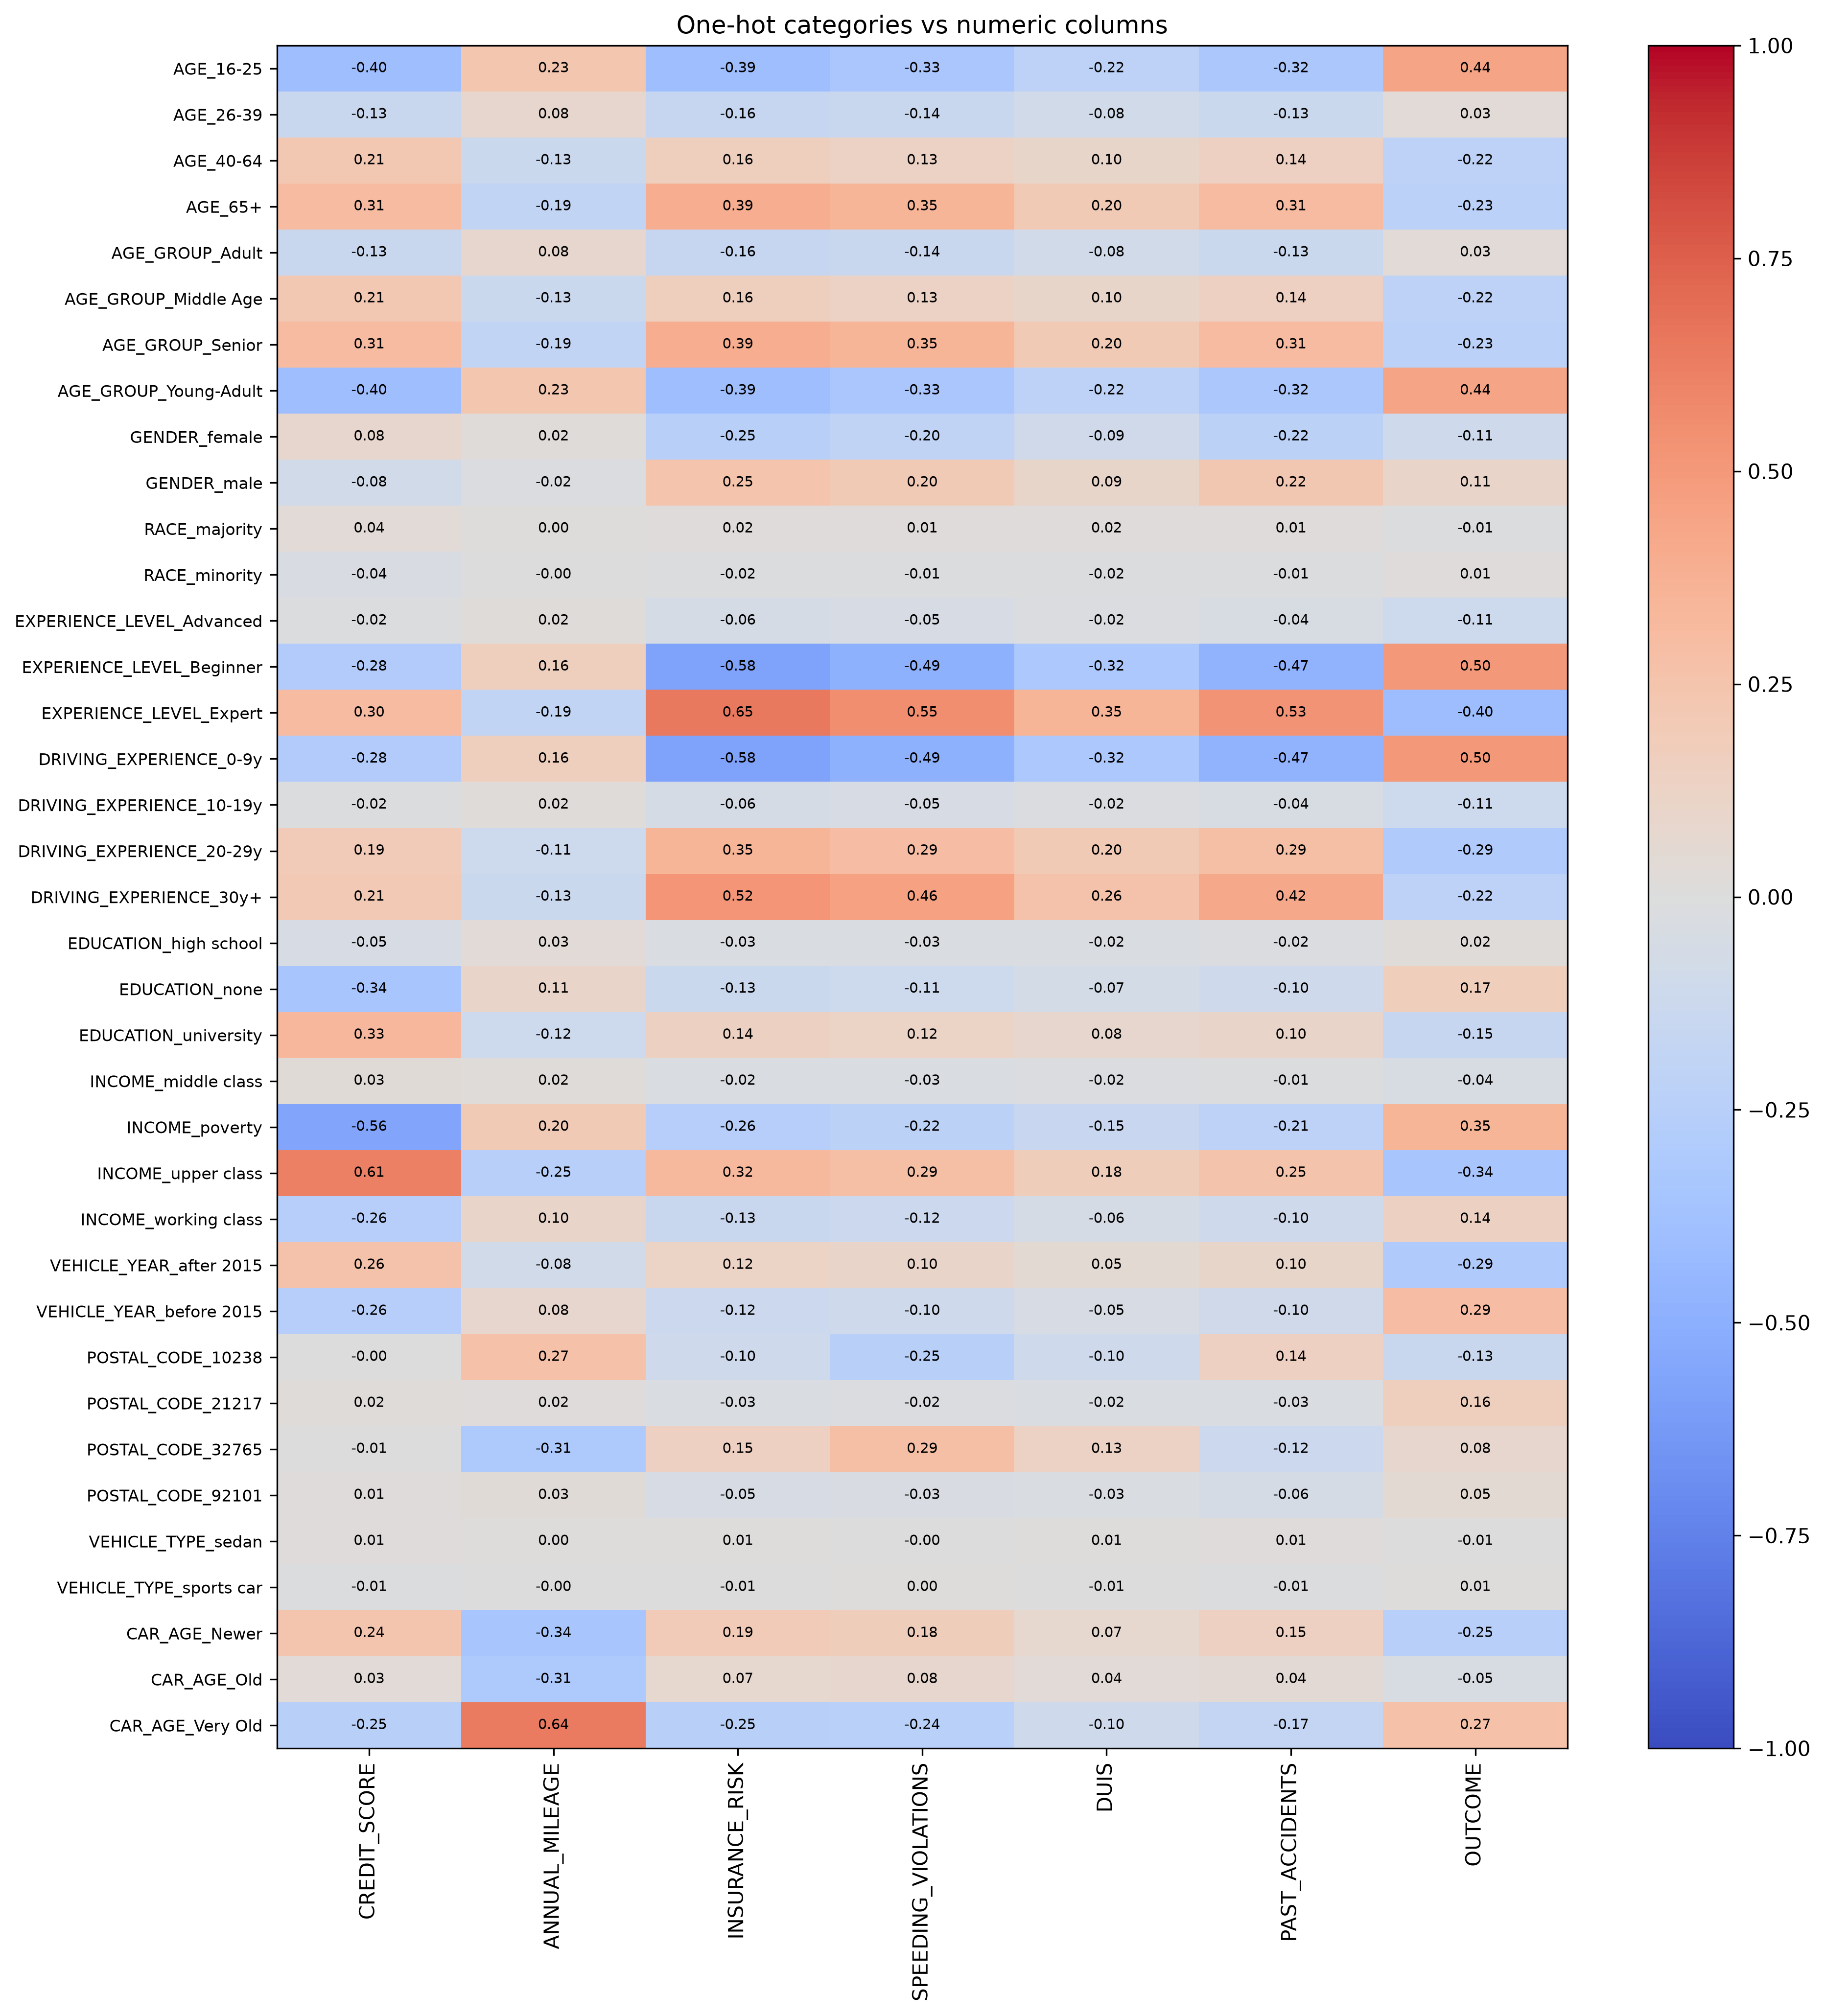
\includegraphics[width=\columnwidth]{onehot_numeric_corr.png}
\caption{Point-biserial correlations between one-hot encoded categories (rows) and the numeric features and target (columns).}
\label{fig:onehot}
\end{figure}

To connect the categorical features to the correlation analysis, each category was one-hot encoded and 
correlated with the numeric columns (Fig.~\ref{fig:onehot}). Dummies were not correlated against each 
other, since mutually exclusive categories of the same variable are negatively correlated by construction. 
The strongest category-level correlations with OUTCOME are listed in Table~\ref{tab:onehot}. 
Drivers with 0--9 years of experience ($r = +0.501$) and drivers aged 16--25 ($r = +0.439$) are the groups 
most associated with filing a claim, while expert drivers ($r = -0.401$) and upper-class income 
($r = -0.339$) are associated with fewer claims.

\end{document}